\begin{subsectionframemod}{Object Detection}
    \metroset{block=fill}
    \vspace{-10mm}
    \begin{alertblock}{Regular Object Detection}
        Given a set of classes $\mathcal{C}$, find all occurences of objects
        belonging to any class $c \in \mathcal{C}$ in an image $I$. Each object is reprented as $(x_1, y_1, x_2, y_2, c)$.
    \end{alertblock}

    \vspace{5mm}
    \pause
    \begin{columns}
        \begin{column}{0.3\textwidth}
            \centering
            \begin{tikzpicture}
                \node[anchor=south west,inner sep=0, label=below:{\small Input image $I$}] at (0,0){
                    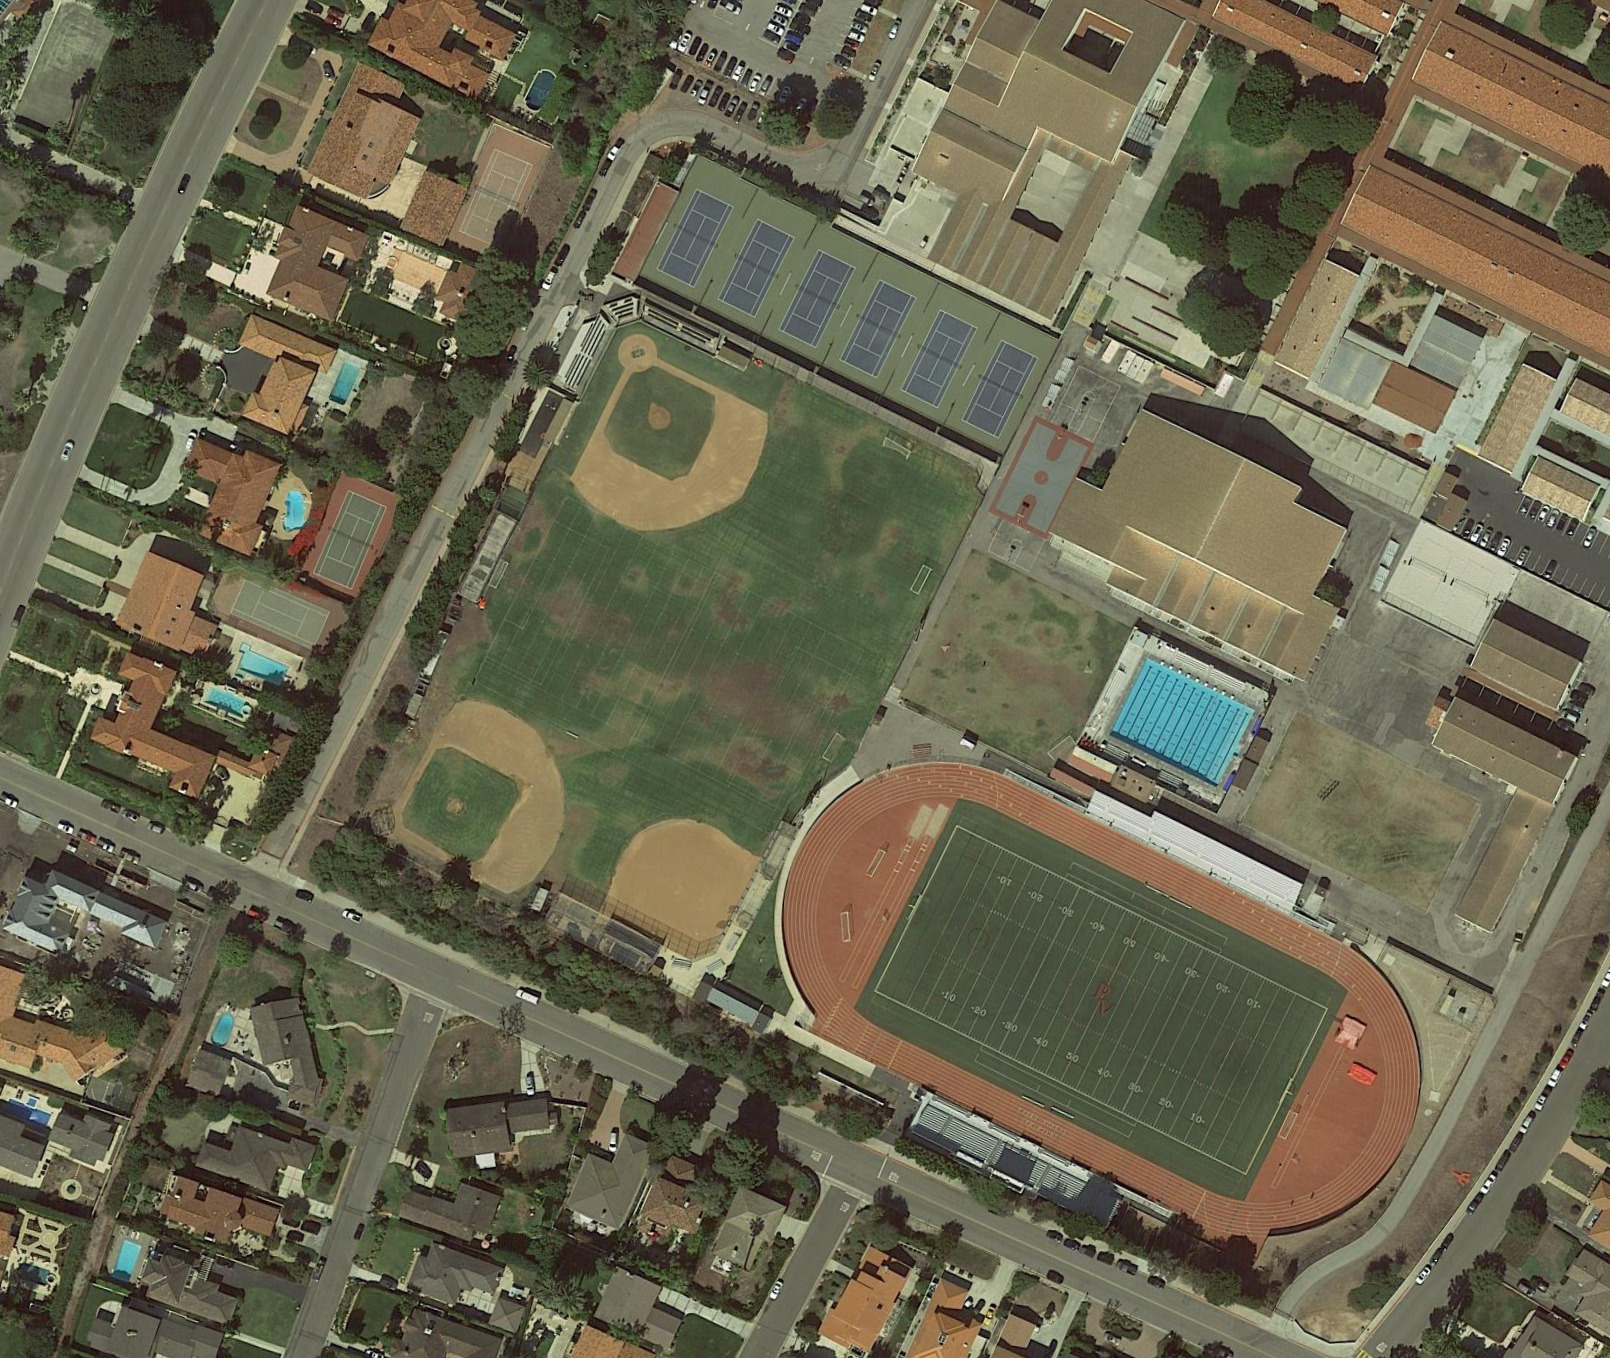
\includegraphics[width=30mm]{Figures/P0770.jpg}
                };
               
            \end{tikzpicture}
            
        \end{column}
        \pause
        
        \begin{column}{0.3\textwidth}
            

            \only<4->{
                \begin{textblock*}{50mm}(41mm,53mm)
                    \huge $\rightarrow$
                \end{textblock*}
                

                \begin{tikzpicture}[remember picture,overlay]
                    \node[xshift=\paperwidth/2 +0mm,yshift=-\paperheight/2- 5.5mm] at (current page.north west){%
                        \fbox{\parbox[][10mm][c]{0.8\textwidth}{\centering\normalsize Detection model}}
                    };
                \end{tikzpicture}
            }
            % \graphicsbox{Figures/P0131.jpg}{(0.2,0.2)}{(0.23,0.5)}{green}[20mm][0.2mm]
        \end{column}
        \pause
        \begin{column}{0.3\textwidth}
            \only<5->{
                \begin{textblock*}{50mm}(82mm,53mm)
                    \huge $\rightarrow$
                \end{textblock*}
                \centering
                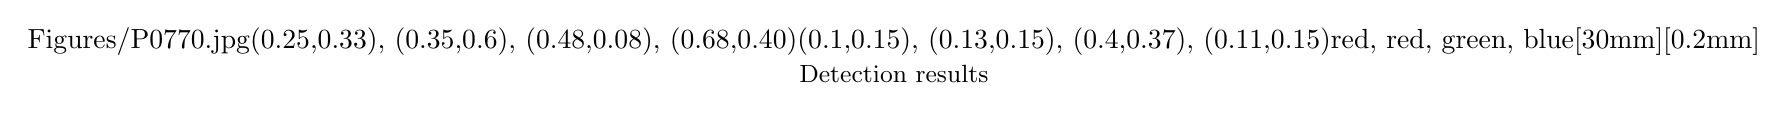
\begin{tikzpicture}
                    \node[anchor=south west,inner sep=0, label=below:{\small Detection results}] at (0,0){
                        \graphicsbox{Figures/P0770.jpg}{(0.25,0.33), (0.35,0.6), (0.48,0.08), (0.68,0.40)}{(0.1,0.15), (0.13,0.15), (0.4,0.37), (0.11,0.15)}{red, red, green, blue}[30mm][0.2mm]
                    };
                
                \end{tikzpicture}
            }
            
        \end{column}
    \end{columns}
    
    \only<3->{
    \begin{textblock}{12}(2, 12)
        $$ \mathcal{C} = \{ \text{Baseball-diamond, Swimming-pool, Ground-track-field} \}$$
      \end{textblock}
    }
        
\end{subsectionframemod}